\chapter{Project Management}

\section{Project Name / Supervisor / Manager }    Project \hspace{2mm} \textemdash \hspace{2mm} InforMe@Dublin
\newline
Supervisor \hspace{2mm} \textemdash \hspace{2mm}  Dr Simon McLoughlin
\newline
Manager \hspace{2mm} \textemdash \hspace{2mm}  Adam O\textquotesingle Connor

\section{Success Criteria}
\begin{itemize}
	\item The complete program should be able to locate their current location and if a building of significant historical value.
	\item The program should allow other users to learn and about their area.
	\item The program also allows the users to explore their town and get fit by doing so.
	\item The application should educate the user and tell them the information.
	\item Program should have great user functionality and work very efficiently for the user.
	\item Should be very user-friendly.
\end{itemize}

\section{Assumptions Risks and Obstacles }
\begin{itemize}
	\item Coding a responsive application for the Android operating system.
	\item Using the Google Maps API and location service's that are incorporated into an android device.
	\item Using Android Studio to create this application.
	\item Coding from scratch and learning new technologies on the way.
	\item Allocating time and resources to develop the application as a whole.
	\item Timekeeping to allow us for the project to be completed within a reasonable time-scale.
\end{itemize}

\section{Motivation for choosing project}
With the influence of new mobile technologies throughout this day and age, the developer has always seen a niche market for an application that utilises and explores the user's town. Everyone has readily available internet connectivity on our mobile phones and if not a GPS module incorporated into that device. With towns growing rapidly throughout the years all the hidden gems of these area's are being left behind with no-one knowing the history of what is there.

A developers job is to either make things easier on people or to produce new idea's or technologies for a normal user to use. The only flaw of this project is the user needs to own an Android device and have an internet connection. The project enables the user to walk around their town and to discover new areas with the use of this app. The app should provide some Wikipedia type adjustments that will be sent to the admin or requests to show lost monuments or where historical relics have been found.

Due to some of the historical finds that have been found around Dublin and some of the structures with the likes of Neolithic axes found as well as the oldest bridge in Ireland that provides passage over the Griffeen Valley River.

\newpage

\section{Methodology}
\textbf{V Model}
The model that we will be using to develop this project will be the V – Model, why the developer chose this model, is because the steps in progress are in a sequential manner in and the type in question is also known as the verification and validation model. Which means after each step is complete, the software and hardware are both Verified and validated.
The model chosen is an augmentation of the waterfall model and is based on the testing of each phase of the development which means each step of the development life-cycle there is then a directly associated testing phase with each part of code. The type of proposed model, as follows, is a highly disciplined model in that the next step only starts on completion of the open phase.
\cite{TPoint}


\begin{figure}[htbp]
	\center 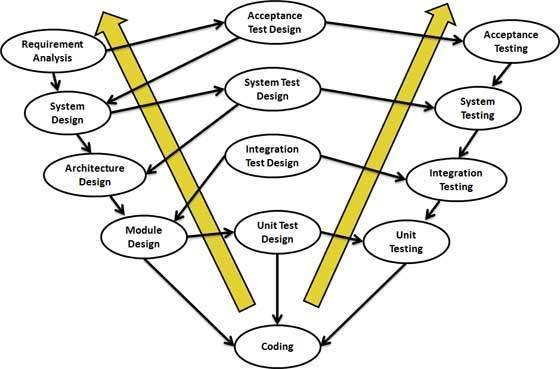
\includegraphics[width=400pt]{vshapedmodel}\\
	\caption{Image of the V Model \citep{TPoint}} \label{Figure: V Shaped Model 
		Area}
\end{figure}

\newpage
\begin{table}[!ht]
	\section{Work Breakdown Structure}
	\begin{tabular}{ l l l }
		\textbf{Objective} && \textbf{Task} \\
		Complete Project Proposal. && Complete within 2 weeks. \\
		Research and test Google maps API and geo-location. && Complete within 1 week. \\
		Research android application development with the cloud. && Complete within 1 week. \\
		Preform literature review on the project. && Complete within 2 weeks. \\
		Risk analysis. && Complete within 2 weeks. \\
		Development plan. && Complete within 1 week. \\
		Build prototype. && Complete within 3 weeks. \\
		Second risk analysis. && Complete within 1 week. \\
		1st validation and verification. && Complete within 1 week. \\
		Operational prototype. && Complete within 1 week. \\
		2nd validation and verification. && Complete within 1 week. \\
		Final development. && Complete within 2 weeks. \\
		Implementation. && Complete within 1 week. \\
	\end{tabular}
	\caption{Table of Work Breakdown Structure.}
	\label{table : Work Breakdown Structure.}
	\newpage
\end{table}

\section{Technologies and Skills Needed}
\begin{enumerate}
	\item Programming  in the Java development language.
	\item Using and incorporating APIs into Android applications.
	\item Knowledge of XML for design layouts.
	\item Knowledge of JSON.
	\item Knowledge of Firebase and its associated methods.
	\item Experience of using Google's developer console.
	\item Experience of developing application's for Android devices.
	\item Using and adapting gradle properties of Android applications.
	\item Underlying architecture of the Android OS.
	\item Utilising modules of the Android Device.
	\item Learning new permission requests of Android Marshmallow and above.
	\item Utilising the battery life of Android devices.
	\item Knowledge of Location Services.
	\item Knowledge of Computational processes of Android devices.
\end{enumerate}

\section{Gantt Chart}
Below is a following gantt chart with regards to the work of which will be completed by the developer throughout the development of such an application of this size.
\begin{figure}[!ht]
	\center 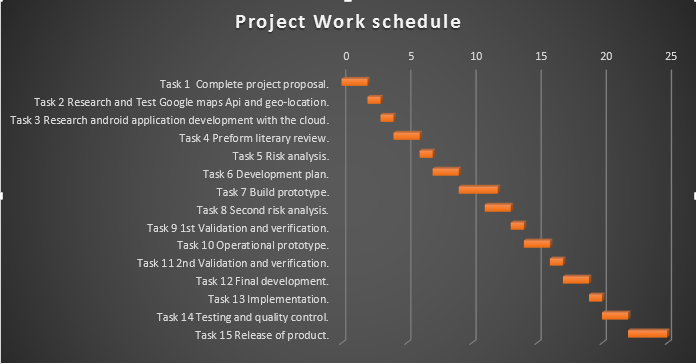
\includegraphics[width=420pt, height=250pt]{ganntChart}\\
	\caption{Gantt Chart} \label{Figure: Gantt Chart of work breakdown structure.  
		Area}
\end{figure}

\newpage

\section{Development Device}
Concerning the development section of the following thesis of which is about the device on which the Android application would be developed on. The device in question is as follows -

\begin{table}[!ht]
	\begin{tabular}{ l l l }
		\textit{Mobile Name} && Alcatel Pop 4+ \\
		\textit{Operating System} && Android 6.0 (Marshmallow)\\
		\textit{CPU} && Quad-core 1.1 GHz Cortex-A7 \\
		\textit{Chipset} && Qualcomm MSM8909 Snapdragon 210 \\
		\textit{RAM} && 1.5GB Ram \\
		\textit{Internal Memory} && 16GB \\
		\textit{Battery} && Removable Li-Ion 2500 mAh battery \\
	\end{tabular}
\caption{Alcatel Pop 4+ Specifications.}
\label{table : Alcatel Pop 4+ Specifications.}
\end{table}

\begin{figure}[!ht]
	\center 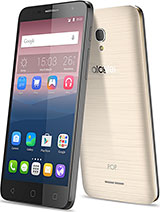
\includegraphics[width=150pt, height=250pt]{alcatel}\\
	\caption{Alcatel Pop 4+} \label{Figure: Alcatel Pop 4+}
\end{figure}

\newpage
\section{Conclusion}
This project as a whole is ready to start. Some changes may occur during the development throughout the build and production. The next stage of the project in the question is to research all available sources and technologies that can be used in the creation of such project. The Finished development of the application scheduled for the end of April 2017, with a mock-up build of the project due in December 2016.
